\documentclass[10pt,a4paper]{article}
\usepackage[utf8]{inputenc}
\usepackage[T1]{fontenc}
\usepackage{graphicx}
\usepackage[usenames, dvipsnames]{xcolor}
\usepackage{float}
\usepackage{mathtools}
\usepackage{amsmath}
\usepackage{amsfonts}
\usepackage{amsthm}
\usepackage{thmtools}
\usepackage{enumitem}
\theoremstyle{definition}
\newtheorem{definition}{Definition}[part]
\newtheorem{subdefinition}{Definition}[definition]

\declaretheorem[sibling=definition, shaded={rulecolor=black, rulewidth=0.8pt, 
	bgcolor={rgb}{1,1,1}},name=Definition]{boxeddef}
\declaretheorem[sibling=subdefinition, shaded={rulecolor=black, rulewidth=0.5pt, 
	bgcolor={rgb}{1,1,1}},name=Definition]{boxedsubdef}

\theoremstyle{plain}
\newtheorem{example}{Example}[definition]


\title{Machine Learning 2023}
\author{David Graf}
\date{\today}
\begin{document}
	\maketitle
\part{Actual ML lecture content}
Recap of our setup:
\begin{enumerate}
	\item DOMAIN set X; we call $x\in X$ an instance
	\item LABEL set Y; e.g. $Y = \{0, 1\}$ (for a binary problem)
	\item TRAINING set $\mathcal{S} = \big((x_1, y_1), ..., (x_m, y_m)\big)$  with $x_i \in X, y_i \in Y$
	\item a LEARNER that receives $\mathcal{S}$ and outputs 
	$$ h: X \to Y$$
	which we call a hypothesis
\end{enumerate}
Assumption: for now, we assume $x_i$'s are drawn iid from some probability measure $\mathcal{D}$ over the domain and labelled by some function (the labelling function) $f: X \to Y$:
$$ x_i \underbrace{ \sim }_{\text{\scriptsize"drawn from"}} \mathcal{D},\ y_i = f(x_i)$$

We are "interested" in 
$$\mathcal{D}(\{x \in X: h(x) \neq f(x) \}) = \mathbb{P}_{X \sim \mathcal{D}}[h(x) \neq f(x)] = L_{\mathcal{D}, f}(h)$$
$L_{\mathcal{D}, f}(h)$ is called the "Generalization Error" or "Risk".\\
\newline
The \underline{empirical version} of this is 
\begin{equation}
	\tag{[m] = \{1, ..., m\}}
	\frac{1}{m}\cdot\big|\big\{ i \in [m]: h(x_i) \neq f(x_i) \big\}\big| = L_\mathcal{S}(h)
\end{equation}
the empirical error or empirical risk $L_\mathcal{S}(h)$.
\paragraph{Convention:}
$\mathcal{S}|_x = (x_1,..., x_m)$

\paragraph{Claim:}
ADD COMMENTS ON THE SIDE HERE, SLIDE 27
\begin{align*}
 \mathbb{E}_{\mathcal{S}|_x \sim \mathcal{D}^m}[L_\mathcal{S}(H)] &= \mathbb{E}_{\mathcal{S}|_x}\bigg[\frac{1}{m} \cdot \sum_{i=1}^{m} 1_{h(x_i) \neq f(x_i)}\bigg]\\
 &= \frac{1}{m} \cdot \sum_{i=1}^{m} \mathbb{E}_{x_i \sim \mathcal{D}}[1_{h(x_i) \neq f(x_i)}] && \text{(by linearity of $\mathbb{E}$)}\\
 &= \frac{1}{m} \cdot \sum_{i=1}^{m} \mathbb{E}_{X \sim \mathcal{D}}[1_{h(x) \neq f(x)}]\\
 &= \frac{1}{m} \cdot \sum_{i=1}^{m} \mathbb{P}_{X\sim \mathcal{D}}[1_{h(x) \neq f(x)}]\\
 &=  \frac{1}{m} \cdot m \cdot \mathbb{P}_{X\sim \mathcal{D}}[1_{h(x) \neq f(x)}]\\
 &= L_{\mathcal{D},f}(h)
\end{align*}

\paragraph{Our first learning paradigm} \underline{Empirical risk minimization (ERM)}:\\
As we only have access to the training data (S), it's natural to try to select \underline{h} such that the empirical risk is minimized. We call such an h an \underline{empirical risk minimizer} $(h_S)$.\\

\underline{A problematic case:}
\begin{figure}[H]
	\centering
	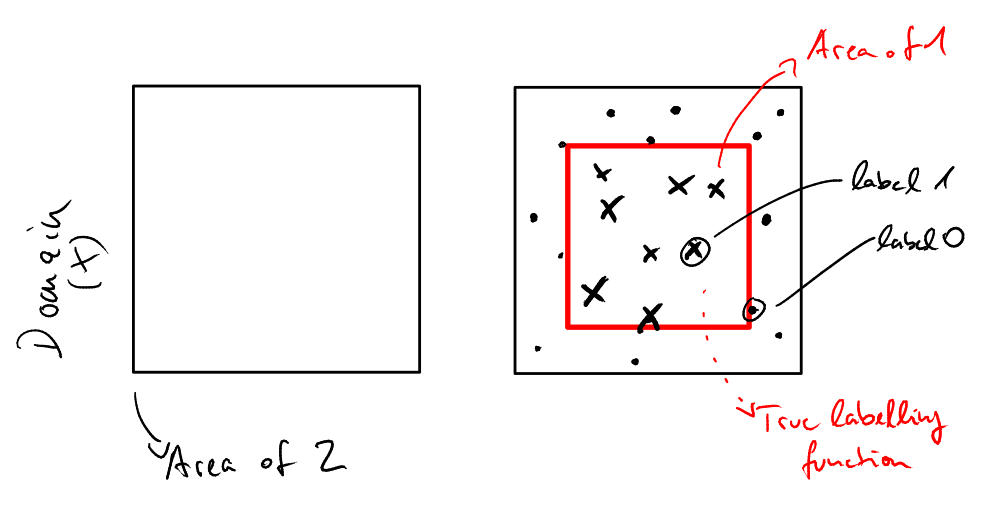
\includegraphics[width=0.7\linewidth]{sketch_1}
	\caption{Problematic Case 1}
	\label{fig:sketch1}
\end{figure}

\begin{itemize}
	\item say the distribution on X is uniform
	\item say we have an ERM algorithm that returns $h_S$ such that 
	\begin{align*}
			 h_s(x) &= \begin{cases}
			y_i , &  \text{if } \exists \ i \in [m]: x_i = x  \\
			0 , &  \text{else} 
		\end{cases} && \text{(a lookup table)} 
	\end{align*}
	Obviously $h_S$ is correct on our training set $$\implies L_S(h_S) = 0\text{ !}$$
	But on unseen instances from $D (X \sim D)$, $h_S$ is only correct 50\% of the time (due to the ratio of the areas of the black and red squares in the sketch): $$\implies L_{D,f}(h_S) = \frac{1}{2} \text{ !}$$
	This is called overfitting.
\end{itemize}

\paragraph{Hypothesis class (H):} We restrict searching for h to H, i.e., a class of functions from X to Y, and write:
$$
\text{ERM} = \text{ERM}_{H} (\mathcal{S}) \in \text{argmin}_{h \in H} L_{\mathcal{S}}(h)
$$
\underline{Remark:} In our previous example, we did not do this and allowed to memorize the training data!

\paragraph{ERM over finite hypothesis classes $(\big|H\big| < \infty)$:} 
$$\text{\underline{Assumption (realizability):} } \exists \ h^*\in H \text{ with } L_{\mathcal{D},f}(h^*) = 0$$
Now, any ERM hypothesis $h_\mathcal{S}$ will attain 0 empirical error ($L_\mathcal{S}(h_\mathcal{S}) = 0$), as it computes with $h^*$ (which obviously has 0 empirical error).\\
\newline
Hence, $L_{\mathcal{D},f}(h_\mathcal{S}) > \varepsilon$ can only happen if we select a hypothesis with $L_\mathcal{S}(h_\mathcal{S}) = 0$ but $L_{\mathcal{D},f}(h_\mathcal{S}) > \varepsilon$ (trivially). We can write
\begin{align*}
	H_\text{\textbf{bad}} = \{h \in H: L_{D,f}(h)>\varepsilon\} && \text{ set of \textbf{bad} hypotheses}
\end{align*}
Also, we define
$$
	M = \{\mathcal{S}|_x : \exists h \in \underbrace{H_{\mathrm{\textbf{bad}}}}_{\mathclap{\text{those are the ones with generalization error $> \varepsilon$}}}, L_\mathcal{S}(h) = 0  \}
$$

We observe
$$
\big\{\mathcal{S}|_x : L_{\mathcal{D},f}(\underbrace{h_\mathcal{S}}_{\mathclap{\text{ERM}}}) \geq \varepsilon\big\} \subseteq  \underbrace{\big\{\mathcal{S}|_x : \exists \ h \in H_{\mathrm{\textbf{bad}}}, L_\mathcal{S}(h) = 0 \big\}}_{\mathclap{M = \cup_{h \in H_{\mathrm{\textbf{bad}}}}\{\mathcal{S}|_x: L_{\mathcal{S}}(h) = 0\} }} = M
$$

We get (upon measuring with $\mathcal{D}$):
\begin{align*}
\mathcal{D}^m \big( \{\mathcal{S}|_x : L_{\mathcal{D},f}(h_\mathcal{S}) \geq \varepsilon\}\big) &\leq \mathcal{D}^m\big( \cup_{h \in H_{\mathrm{\textbf{bad}}}}\{\mathcal{S}|_x : L_{\mathcal{S}}(h) = 0\} \big)\\
&\leq \sum_{h \in H_{\mathrm{\textbf{bad}}}} \mathcal{D}^m \big(\{\mathcal{S}|_x : L_{\mathcal{S}}(h) = 0\}\big) && \text{(due to $\sigma$-sub-additivity)}
\end{align*}
\underline{Let's fix some $h \in H_{\mathrm{\textbf{bad}}}$:}
\begin{align*}
	D^m \big(\{\mathcal{S}|_x : L_{\mathcal{S}}(h) = 0\}\big) &= \mathcal{D}^m \big(\{\mathcal{S}|_x : \forall i \in [m]: h(x_i) = f(x_i)\}\big)\\
	&= \prod_{i = 1}^{n} \mathcal{D} \big(\{x_i: h(x_i) = f(x_i)\}\big) && \text{(due to iid assumption)}\\
	&= \prod_{i=1}^{n} (1 - L_{\mathcal{D},f}(h))\\
	&\leq \prod_{i=1}^{n} (1-\varepsilon) && \text{(as $h \in H_{\mathrm{\textbf{bad}}}$)}\\
	&= (1-\varepsilon)^m \\
	&\leq e^{-\varepsilon m}
\end{align*}
So, to conclude:
\begin{align*}
	D^m \big(\{\mathcal{S}|_x : L_{\mathcal{D},f}(h_S) \geq \varepsilon\}\big) &\leq \sum_{h \in H_{\mathrm{\textbf{bad}}}} e^{-\varepsilon m} \\ 
	&= |H_{\mathrm{\textbf{bad}}}| \cdot e^{-\varepsilon m} \\
	&\leq |H| \cdot e^{-\varepsilon m}
\end{align*}
This is a probabilistic guarantee that tells us how the generalization error scales with the sample size. If we increase m, ew can make $\varepsilon$ arbitrarily small. 
If we let $ |H| \cdot e^{-\varepsilon m} <\delta \in (0,1)$ and solve for $m$, we get 
$$ m>\frac{1}{\underbrace{\colorbox{orange}{$\varepsilon$}}_{error}} \cdot \log \Big(\frac{|H|}{\underbrace{\colorbox{orange}{$\delta$}}_{confidence}}\Big)$$
\paragraph{Corollary:} Let $|H| < \infty$ and $\varepsilon, \delta \in (0,1)$. Let $m$ be an integer (the sample size) such that $\color{red} m>\frac{1}{\varepsilon} \cdot log \big(\frac{|H|}{\delta}\big)$. Then, for each labeling function $f: X \to Y$ and any distribution $\mathcal{D}$ over domain $X$ (for which realizability holds), we have that with probability of at least $1-f$ over the choice of $S|_x$ (of size m) it holds that every ERM hypothesis $h_s$ satisfies the following:
$$ L_{\mathcal{D},f} \leq \varepsilon $$

\textcolor{red}{\paragraph{Interpretation:} For sufficiently large $m, ERM_H$ returns $h_S$ (i.e., a hypothesis) that is \textbf{P}ROBABLY \textbf{A}PPROXIMATELY \textbf{C}ORRECT (PAC).}\\
\newline
This leads to:
\begin{boxeddef}[PAC learnability]
	A hypothesis class $H$ is \textcolor{red}{PAC learnable}, if there exists a function $m_H: (0,1)^2 \to \mathbb{N}$ and a learning algorithm $\mathcal{A}$ with the following properties:
	\begin{enumerate}
		\item for every $\varepsilon, \delta \in (0,1)$ and
		\item every distribution $\mathcal{D}$ over domain $\mathcal{X}$ and
		\item every labelling function $f: X \to \{0, 1\}$ if
		\item realizability holds (w.r.t. to $\mathcal{D}, H, f$) then
	\end{enumerate}
	running $\mathcal{A}$ on $m \geq m_H(\varepsilon, \delta)$ \textit{iid.} instances drawn from $\mathcal{D}$ and labelled by $f$, returns a hypothesis $h$ such that with probability of at least $1-\delta$ (over choice of S) 
	$$ L_{\mathcal{D}, f} \leq \varepsilon $$
\end{boxeddef}
\begin{boxedsubdef}[Sample complexity]
	$m_H: \{0,1\} \to \mathbb{N}$ is called the \textcolor{red}{sample complexity} function. In particular, $m_H$ returns the smallest integer such that the requirements for PAC-learnability are satisfied
\end{boxedsubdef}
We have already seen that \textcolor{red}{finite hypothesis classes} ($|H| < \infty$) \textcolor{red}{are PAC learnable} with 
$$ m_H(\varepsilon, \delta) \leq \bigg\lceil\frac{1}{\varepsilon} \cdot log \bigg( \frac{|H|}{\delta}\bigg) \bigg\rceil $$

We will now move to a more general setting.
\begin{enumerate}[label*=\protect\fbox{\arabic{enumi}}]
	\item We will first release the realizability assumption (In this setting, the best we can hope for are guarantees relative to the "best" possible hypothesis in the class: $$\min_{h \in H}{L_{\mathcal{D}, f}(h)}$$
\end{enumerate}
	\begin{boxeddef}[Höffding inequality]
	Let $X_1, ..., X_m$ be \textit{iid} random variables taking values in $[a_i, b_i]$ for $i \in [m]$. Then, it holds that
	 \begin{align*}
	 	\mathbb{P}\left[S_m - \mathbb{E}[S_m] > \varepsilon\right] &\leq e^{\left(\frac{-2 \varepsilon^2}{\sum_{i} (b_i - a_i)^2}\right)} && ; S_m = \sum_{i = 1}^{m} X_i, \text{ and}\\
	 	\mathbb{P}\left[S_m - \mathbb{E}[S_m] < -\varepsilon\right] &\leq e^{\left(\frac{-2 \varepsilon^2}{\sum_{i} (b_i - a_i)^2}\right)} 
	\end{align*}
	Also:
	\begin{align*}
	 	\mathbb{P}\bigg[\big|S_m - \mathbb{E}[S_m]\big| > \varepsilon\bigg] &\leq 2 \cdot e^{\frac{-2 \varepsilon^2}{\sum_{i} (b_i - a_i)^2}}\\
	 	HIER NOTIZ EINFÜGEN
	 \end{align*}

\end{boxeddef}
Another useful form of this inequality is:
$$ \mathbb{P} \left[\left| \frac{1}{m} \cdot \sum_{i = 1}^{m} X_i - \mu \right| \geq \varepsilon\right] \leq 2 \cdot e^{\frac{-2 \varepsilon^2 m}{b-a}} $$
with $\mu = \mathbb{E}[X_i]$ and $\mathbb{P}[a \leq X_i \leq b] = 1$ for all $i \in [m]$. As a consequence, we can say the following: fix $\varepsilon>0$; then for any \colorbox{Apricot}{\underline{single} $h: X \to Y$}, we have 
$$ \mathbb{P}_{S|_x \sim \mathcal{D}^m}\left[\left|L_{s}(h) - L_{\mathcal{D}, f}\right| > \varepsilon\right] \leq 2 e^{-2\varepsilon^2 m} \hspace{1cm} (a = 0, b = 1)$$
If we would set $\delta = 2^{-2 \varepsilon^2 m}$, and solve for $\varepsilon$, we would get
\begin{align*}
\varepsilon &= \sqrt{\frac{log\big(\frac{2}{\delta}\big)}{2m}}\\
\implies L_{\mathcal{D},f}(h) &\leq L_{s}(h) + \sqrt{\frac{log\big(\frac{2}{\delta}\big)}{2m}}\\
\text{\textcolor{red}{(holds with probabilty of }} & \text{\textcolor{red}{at least $1-\delta$ over choice of S)}}
\end{align*}
\paragraph{Remark:} This result holds for a \underline{single} h. However, we can easily get a bound that holds \underline{uniformly} for all $h \in H, |H| < \infty$
$$ \mathbb{P}_{S|_x \sim \mathcal{D}^m} \bigg[\exists h \in H: \big|L_{s}(H) - L_{\mathcal{D}, f}(h) \big| > \varepsilon \bigg] \leq \sum_{h \in H} 2\cdot e^{-2 \varepsilon^2 m} \leq 2 \big|H\big| \cdot e^{-2 \varepsilon^2 m} $$ 
We will see that we did need realizability for that!

\begin{enumerate}
	\item[\protect\fbox{2}] Next, we release our requirement of a "true" labelling function $f$. We do this by letting $\mathcal{D}$ be a distribution over $\mathcal{X} \times \mathcal{Y} = \mathcal{Z}$. We need to adjust our definitions of empirical error and generalization error:
	\begin{eqnarray}
		L_{\mathcal{D}}(h) = \mathbb{P}_{(x, y) \sim \mathcal{D}}
	\end{eqnarray}
\end{enumerate}
Both \protect\fbox{1} and \protect\fbox{2} lead to:
\begin{boxeddef}[Agnostic PAC learnability]
	A hypothesis class $H$ is \textcolor{red}{agnostic PAC learnable}, if there exists a function $m_H: (0,1)^2 \to \mathbb{N}$ and a learning algorithm $\mathcal{A}$ with the following properties:
	\begin{enumerate}
		\item for every $\varepsilon, \delta \in (0,1)$ and
		\item every distribution $\mathcal{D}$ over domain $\mathcal{X} \times \mathcal{Y}$
	\end{enumerate}
	running $\mathcal{A}$ on $m \geq m_H(\varepsilon, \delta)$ \textit{iid.} instances drawn from $\mathcal{D}$, returns a hypothesis $h$ such that with probability of at least $1-\delta$ (over choice of S) 
	\textcolor{red}{$$ 
		L_{\mathcal{D}}(h) \leq \min_{h' \in H} L_{\mathcal{D}}(h') + \varepsilon
		$$}
\end{boxeddef}
Implicit assumption: the best possible thing from the hypothesis class is at least okay. If it is large, then the min is large, and consequently the threshold is bad!\\
To show that \textit{finite classes are agnostic PAC learnable}, we will use the Höffding inequality.

\paragraph{General loss functions}
	$$ l: H \times (X \times Y) \rightarrow \mathbb{R}_+ $$
Example: \textcolor{red}{0-1 loss}\\
$$ l^{0-1}\left( h, \left(x,y\right) \right) = \begin{cases}
	1, &  \text{if } h(x) \neq y  \\
	0, &  \text{else} 
\end{cases}$$

\textcolor{red}{square loss:}
\begin{align*}
l^{sq}(h, \underbrace{\left(x,y\right)}_{\text{e.g.} \in \mathbb{R}}) =  \left(y-h(x)\right)^2 & \hspace{3cm} \text{\textit{e.g. in regression problems}}
\end{align*}
In case of general loss functions, we adjust our definitions of $L_\mathcal{D}$ and $L_\mathcal{S}$ as follows:
$$ 
L_\mathcal{D}(h) =  \mathbb{E}_z[l(h, z)], \ \  L_\mathcal{S}(h) = \frac{1}{m} \cdot \sum_{i = 1}^{m} l(h, z_i)
$$

\paragraph{Remark:}
$$
\mathbb{E}_z\left[l^{0-1}(h,z)\right] = 0 \cdot \mathbb{P}_z[h(x) = y] + 1 \cdot \mathbb{P}_z[h(x) \neq y] = \mathbb{P}_z[h(x) \neq y]
$$

\section*{Uniform convergence}
\begin{boxeddef}[$\varepsilon$-representative sample]
	A sample S is called \textcolor{red}{$\varepsilon$-representative sample} wrt. $\mathcal{Z} (= \mathcal{X}\times\mathcal{Y})$, loss function $l$ and distribution $\mathcal{D}$, if
	$$
	\forall h \in H: \left|L_S(h) - L_\mathcal{D}(h)\right| \leq \varepsilon
	$$
\end{boxeddef}
\paragraph{Lemma:} Assume that S is $\frac{\varepsilon}{2}$-representative wrt. $\mathcal{Z}, H, l$ and $\mathcal{D}$. Then, any hypothesis \textcolor{red}{$h_S$} returned by $ERM_H(S) \in argmin_{h' \in H}(L_\mathcal{S}(h'))$ satisfies
$$
	L_D(\text{\textcolor{red}{$h_S$}}) \leq \min_{h \in H} L_D(h) + \varepsilon
$$

\begin{proof}
for \colorbox{Apricot}{any} $h \in H$:
\begin{align*}
	L_\mathcal{D}(h_s) &\leq L_S(h_S) + \frac{\varepsilon}{2}  \tag{by def. $\varepsilon$-representativeness}\\
	&\leq L_S(h) + \frac{\varepsilon}{2} \tag{as $h_S$ is ERM-hyp.}\\
	&\leq L_\mathcal{D}(h) + \frac{\varepsilon}{2} + \frac{\varepsilon}{2} \tag{by def. $\varepsilon$-representativeness}\\
	&\leq  L_\mathcal{D}(h) + \varepsilon
\end{align*}
As this inequality chain holds for any $h \in H$, we conclude that $$L_\mathcal{D}(h_S) \leq \min_{h \in H} L_\mathcal{D}(h) + \varepsilon$$
\end{proof}
This leads us to the definition of uniform convergence:
\begin{boxeddef}[Uniform convergence]
	A hypothesis class $H$ has the \textcolor{red}{uniform convergence (UC)} property (wrt. $\mathcal{Z}$ and loss function $l$) if there exists\\
	 $m_H^{UC}: (0,1)^2 \rightarrow \mathbb{N}$ such that for every $\varepsilon, \delta \in (0,1)$ and every distribution $\mathcal{D}$ over $\mathcal{Z}$, if $\mathcal{S}$ is an iid sample of size $m > m_H^{UC}(\varepsilon, \delta)$ from $\mathcal{D}$, then with probability of at least $1-\delta$ (over the choice of $\mathcal{S}$), $\mathcal{S}$ is $\varepsilon$-representative
\end{boxeddef}
\paragraph{Corollary:} if $H$ has the UC property with $m_H^{UC}$, then $H$ is agnostic PAC learnable with 
$$
	m_H(\varepsilon, \delta) \leq m_H^{UC}(\frac{\varepsilon}{2}, \delta)
$$
\colorbox{Apricot}{LETZTE ZEILE FEHLT}

\paragraph{Claim:} Finite $H$ ($|H|< \infty$) are agnostic PAC learnable.\\
Given fixed $\varepsilon, \delta \in (0,1)$, we want to show that
$$
	D^{m}\Big(\big\{\mathcal{S}: \forall h \in H: \left|L_S(h) - L_D(h) \right| \leq \varepsilon\big\}\Big) \geq 1-\delta
$$
Equivalently, 
$$
	D^{m}\Big(\big\{S: \exists h\in H: \big|L_S(h)-L_D(h)\big|\textcolor{red}{>}\ \varepsilon \big\}\Big) < \delta
$$
KOMMENTAR ZUR UNION EINFÜGEN
We bound
$$
	D^{m} (UNION) \leq \sum_{h \in H} 
$$
HIER BEARBEITEN\\

\begin{proof}
	Lets fix $ l = l^{0-1}$. As we know that 
$$
	L_D(h) = \mathbb{E}(l(H, z))
$$ and 
$$
	L_s(h) = \frac{1}{m} \sum_{i = 1}^{m} l(h, z_i),
$$
we can use Höffding's inequality (with $b = 1, a=0$):

$$
	D^{m}(\{ S: \exists h \in H: |L_S(h) - L_D(h)| > \varepsilon\}) \leq \sum_{h \in H} 2 \cdot e^{-2 \varepsilon^2 m} = 2 \cdot |H| \cdot  e^{-2 \varepsilon^2 m}
$$
Let $e^{-2 \varepsilon^2 m}$ be smaller than $\delta$, i.e.,
$$
	2 \cdot |H| \cdot  e^{-2 \varepsilon^2 m} < \delta \leftrightarrow m > \log\left( \frac{2 \cdot |H|}{\delta}\right)\cdot \frac{1}{2 \varepsilon^2}
$$
This gives us the \underline{sample complexity function} $m_{H}^{UC}$ for uniform convergence. In other words, for l: $H \times Z \rightarrow [0,1]$, we have 
EINFÜGEN\\

and by our earlier corollary we get for the sample complexity function $m_H$ for \underline{agnostic PAC learnability} 
$$
	m_H(\varepsilon, \delta) \leq m_H^{UC}\left(\frac{\varepsilon}{2}, \delta\right) \leq \left\lceil \frac{2 \cdot \log\left(\frac{2\cdot |H|}{\delta}\right)}{\varepsilon^2} \right\rceil
$$
This establishes the claim.
\end{proof}
The first case that causes problems with this definition:
\begin{figure}[H]
	\centering
	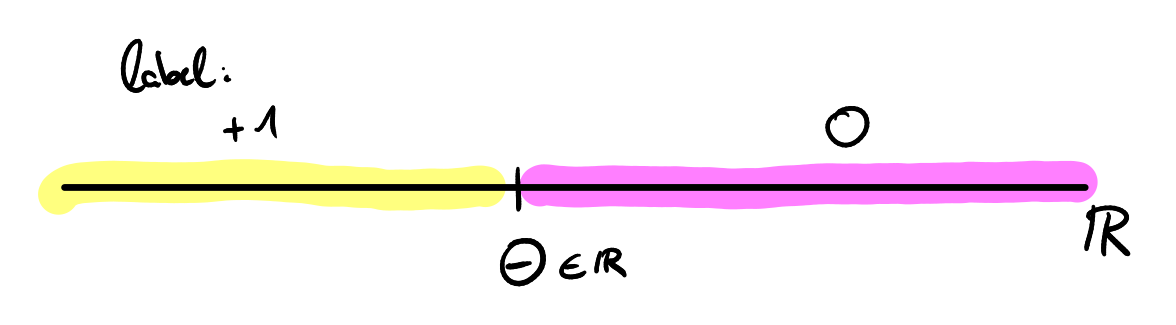
\includegraphics[width=0.7\linewidth]{sketch_2}
	\caption{Problematic Case 2}
	\label{fig:sketch2}
\end{figure}

\end{document}